\documentclass[aps,prl,reprint,amsmath,amssymb]{revtex4-1}

\usepackage{epsfig,color,graphicx}
%\usepackage{algorithmic}
\usepackage{algorithm}
\usepackage{algpseudocode}
\usepackage{soul}
\setcitestyle{super}

% Mathematical symbols
\newcommand*{\imi}{i} % imaginary i
\newcommand*{\E}{\mathrm{e}}
% DIRAC NOTATION
% bra-ket vectors
\newcommand{\ket}[1]{\ensuremath{\vert #1 \rangle}}
\newcommand{\bra}[1]{\ensuremath{\langle #1 \vert}}
\newcommand{\braket}[2]{\ensuremath{\langle #1 \vert #2 \rangle}} % bra-ket inner product
\newcommand{\ketbra}[2]{\ensuremath{\vert #1 \rangle \langle #2 \vert}} % ket-bra outer product
% operators
\newcommand{\op}[1]{\ensuremath{\hat{#1}}} % operator


\makeatletter
\renewcommand\NAT@biblabelnum[1]{{(#1)}}
\makeatother

%text color
%\newcommand{\new}{\color{red}}
%\newcommand{\blue}{\color{blue}}
%\newcommand{\old}{\color{black}}

\begin{filecontents*}{NLMOs-ctrl.bib}
@Control{achemso-ctrl,
  ctrl-article-title = {yes}
}
\end{filecontents*}

\begin{document}
\nocite{achemso-ctrl}

\bibliographystyle{achemso}

\title{
Nonorthogonal  occupied and virtual orbitals
}

\author{Ziling Luo}
\email{ziling.luo@mail.mcgill.ca}
\author{Rustam Z. Khaliullin}
\email{rustam.khaliullin@mcgill.ca}
\affiliation{Department of Chemistry, McGill University, 801 Sherbrooke St. West, Montreal, QC H3A 0B8, Canada}

\date{\today}

\begin{abstract}

\end{abstract}


\maketitle

\section{Introduction} 
Spatially localized orbitals are widely used in electronic structure theory.
Occupied localized orbitals help describe, visualize and classify chemical bonding between atoms thus facilitating our understanding of electronic-structure origins of observed properties of atomistic systems.~\cite{boys1960construction, edmiston1963localized, pipek1989fast, niessen1972density, weinhold2012natural}.
Occupied and virtual localized orbitals are crucial ingredients in all local electronic structure methods including Kohn-Sham density functional theory (DFT)~\cite{goedecker1994efficient, bowler2012methods, zalesny2011linear, pulay1986orbital, saebo2001low, pisani2005local, hampel1996local, forner1997numerical} and wavefunction-based electron correlation methods~\cite{saebo1993local, schutz1999low, hetzer2000low, schutz2001low}.
In these methods, it is the locality of one-electron orbitals that allows to dramatically reduce the computational cost of modeling of large systems.

Spatially localized orbitals are known as localized molecular orbitals (LMOs) in the field of molecular quantum chemistry and maximally localized Wannier functions (MLWFs) in solid state physics and materials science~\cite{marzari2012maximally}.
Here, they will be collectively referred to as LMOs whereas the eigenstates of the effective one-electron Hamiltonian will be called canonical molecular orbitals (CMOs) regardless of whether the system is isolated or treated with periodic boundary conditions.

Traditionally, LMOs are constructed by finding the unitary transformation of occupied or virtual CMOs that minimizes the spread of individual orbitals.
Multiple functions have been proposed to perform the orbital localization in molecular systems, such as Boys-Foster~\cite{boys1960construction}, Edmiston-Ruedenberg~\cite{bytautas2002electron, bytautas2003split, edmiston1963localized}, Pipek-Mezey~\cite{pipek1989fast}, and Von Niessen~\cite{niessen1972density}.
The Boys-Foster~\cite{boys1960construction} and Pipek-Mezey~\cite{pipek1989fast} localization functions are considered as two most popular and widely implemented methods, which are based on completely different approach to measure the orbital spreads.
The Boys-Foster scheme is determined by minimizing the the sum of orbital variance and known for simply physical interpretation and low computational complexity.
The Pipek-Mezey localization function, which maximized the sum of the squared atomic charges~\cite{mulliken1955electronic, lowdin1950non, lehtola2014pipek} of individual orbitals, provides a better bonding pattern explanation for orthogonal LMOs~(OLMOs) due to it preserves the $\sigma$-$\pi$ orbital separation during the orbital localization.
The recent study has surprisingly shown that a pair of $\sigma$ and $\pi$ bonds tend to generated mixed $\tau$ and $\tau'$ orbitals for nonorthogonal LMOs~(NLMOs).
Both Boys-Foster and Pipek-Mezey schemes generate reasonable localized occupied orbitals, while recent study has suggested that Pipek-Mezey scheme may produce semilocal orbitals in the case of virtual orbitals~\cite{hoyvik2013pipek} due to the system and basis set dependence property of the localization function.
More advanced Boys-Foster function have been proposed to further localize orbitals and reduce tails, especially for virtual orbitals.~\cite{jansik2011local, hoyvik2012orbital} 
In the case of the $\Gamma$-point approximation of the Brillouin zone for electronic structure calculations with period boundary conditions, the MLWF, which is the condensed matter equivalent representation of LMOs, have been proposed to construct through several successful and efficient optimization schemes~\cite{marzari2012maximally, resta1998quantum, resta1999electron, silvestrelli1999maximally, berghold2000general, jonsson2017theory}.

Since the unitary transformation preserves the orbital metric, orthogonal LMOs~(OLMOs) are obtained through this approach due to the CMOs are orthogonal.
Thus OLMOs tend to have orthogonalization tails, which exhibit as small non-zero values far away from the localization center.
The tails not only reduce the orbital locality but also complicate the interpretation of chemically relevant electronic-structure information which reduce its transferability from one system to another.
To mitigate the undesirable orthogonality effects, metric-preserving unitary transformation has been applied to nonorthogonal orbitals~\cite{hoyvik2017generalising}.
More general variable-metric non-singular transformation ~\cite{anderson1968self, diner1968fully, magnasco1974localized, payne1977hartree, mehler1977self, feng2004An_efficient, cui2010efficient} has been proposed to further lifts the orthogonality constraint and increase the number of degrees of freedom available to localize molecular orbitals.
The NLMOs have been proved to be more localized and have noticeable less tails than corresponding OLMOs.~\cite{feng2004An_efficient, liu2000nonorthogonal}.

Despite substantial efforts haven been made to construct NLMOs~\cite{feng2004An_efficient, liu2000nonorthogonal, peng2013effective, hoyvik2017generalising}, the existing methods either produce NLMOs which are still similar to OLMOs~\cite{sundberg1979variationally} or lead to the linear dependence between the orbitals~\cite{feng2004An_efficient}.
To overcome the linear dependence problem, Yang and co-workers~\cite{feng2004An_efficient, cui2010efficient} have developed a localization method in which the centers of NLMOs are fixed during the minimization of the localization function. 
A new approach has recently been proposed to perform direct unconstrained variable-metric localization of occupied orbitals that allows to obtain NLMOs without pre-determining the orbital centers.~\cite{luo2020direct} 

The crucial step to obtain the LMOs is the optimization of the localization functions, which is conventional achieved by simple Jacobi rotations~\cite{edmiston1963localized, barr1975improved} or exponential~\cite{berghold2000general} or Cayley parameterization of unitary transformations combined with line search methods.
The Jacobi rotations, which are based on consecutive two-by-two rotations of orbitals pairs, are able to properly localize occupied orbitals, but the optimization process may be slow and converge to nonoptimal solutions, especially for large and complicated systems.
Furthermore, the Jacobi rotations might not work at all in the case of virtual orbitals.

The line search methods have been found to be more efficient than the two-by-two orbital transformation for occupied orbitals, even for the simplest steepest descent approach~\cite{edmiston1965localized}.
The conjugate gradient methods, which also predict the new direction only based on the gradient, fail to significantly improve the efficiency compared with the steepest descent method as initially expected.~\cite{ryback1978application}
Multiple second-order methods have also been suggested to accelerate the localization process of occupied orbitals by using the information from the gradient and hessian.~\cite{leonard1982quadratically, kari1984parametrization}
Even though the Hessian involved methods are more time consuming compared with first-order methods, they successfully reduce the necessary amount of iterations by 1-2 orders of magnitude~\citet{leonard1982quadratically}.
The Quasi-Newton methods such as Broyden-Fletcher-Goldfarb-Shanno~(BFGS) algorithm have also been implemented to localize molecular orbitals.~\cite{kari1984parametrization}

Due to the fact that there are multiple not well separated local minimum of the localization functions in the case of virtual orbitals~\cite{subotnik2005fast}, convergence is slow and painful for both first-order and second-order line search methods.
Moreover, the negative Hessian eigenvalues in the initial iterations of orbital localization prevent correctly predicting new directions, therefore the line search methods may fail in the early stage of the optimization process.

More recently, the trust region methods have been demonstrated as an ideal optimization algorithm to localize both occupied and virtual orbitals with various localization functions.~\cite{jansik2011local, hoyvik2012trust, hoyvik2012orbital,hoyvik2013pipek}
However, the comparison between different localization functions has suggested the virtual orbitals obtained by Boy-Foster and Pipek-Mezey schemes are less localized than more advanced and complicated localization schemes.~\cite{hoyvik2013localized} 

Multiple optimization methods have also been implemented for localizing nonorthogonal orbitals.
The trust region methods have successfully applied to metric-preserving nonorthogonal occupied and virtual orbitals.~\cite{hoyvik2017generalising}
The line search methods such as conjugated gradient~\cite{liu2000nonorthogonal}, the Newton method~\cite{feng2004An_efficient} and BFGS method~\cite{cui2010efficient} have been suggested to localize variable-metric nonorthogonal occupied orbitals.

In this work, we designed, tested and compared a variety of line search and trust region algorithms to perform direct unconstrained variable-metric localization of occupied and virtual orbitals. [Currently, there are no reports/methods for variable-metric localization of virtual orbitals (is it true?). Here, we do not only discuss optimization algorithms but also compare, for the first time, virtual NLMOs generated with Boys and PM localization functions.]


\section{Methodology}
\subsection{Theory and Implementation}
In this work, the conventional tensor notation is used to work with the nonorthogonal orbitals~\cite{head1998tensor}: covariant quantities are denoted with subscripts, contravariant quantities with superscripts and summation is implied over the same covariant and contravariant orbital indices. Summation is not implied if two indices are both covariant. 

In order to obtain a set of nonorthogonal localized molecular orbitals, the conventional localization function $\Omega_L$ has been suggested to eliminates unphysical states with linearly dependent orbitals by introducing a penalty function  $\Omega_P$.~\cite{luo2020direct} 
%
\begin{equation} \label{eq:fun-overall}
\begin{split}
\Omega = \Omega_L + c_P \Omega_P, \\
\end{split}
\end{equation}
%
where $c_P > 0$ is the penalty strength.
The NLMOs $\ket{i}$ are expressed as a linear combination of one-electron states $\ket{j_0}$

%
\begin{equation}
\begin{split}
\ket{i} = \ket{j_0} {A^j}_i 
\end{split}
\end{equation}
%
The initial occupied one-electron states are not required to be canonical or orthogonal but need to be normalized and linearly independent, which both preserve the generality of the method and guarantee the overlap matrix is invertible. The initial virtual orbitals are randomly generated followed by projecting out the occupied subspace and orthogonalization.

The Berghold localization function~\cite{resta1998quantum, resta1999electron, berghold2000general}  adopted in this work is equivalent to the Boys-Foster localization scheme~\cite{berghold2000general, resta1999electron} for gas-phase system and only able to describe the electronic states within the  $\Gamma$-point approximation for periodic system:
%
\begin{equation} \label{eq:fun-loc}
\begin{split}
\Omega_L(\mathbf{A}) &= - \sum_K \sum_i \omega_K \vert z_{i}^{K} \vert^2, \\
z_{i}^{K} &= {A^m}_i B^{K}_{mn} {A^n}_i, \\
B^{K}_{mn} &= \bra{m_0} \E^{\imi \mathbf{G}_K \cdot \mathbf{\op{r}}} \ket{n_0}
\end{split}
\end{equation}
%
where $\mathbf{\op{r}}$ is the position operator in three dimensions, $\omega_K$ and $\mathbf{G}_K$ are suitable sets of weights and reciprocal lattice vectors, respectively, labeled by index $K$~\cite{silvestrelli1999maximally, berghold2000general}. 

We also implement the Pipek-Mezey localization function~\cite{pipek1989fast,lehtola2014pipek} to investigate and compare the locality of virtual NLMOs generated with Boys-Foster and Pipek-Mezey localization functions.:
%
\begin{equation} \label{eq:pipek}
\begin{split}
\Omega_L^{\text{PM}}(\mathbf{A}) &= - \sum_{K=1}^{\text{Atoms}} \sum_i \vert z_{i}^{K} \vert^2, \\
z_{i}^{K} &= {A^m}_i B^{K}_{mn} {A^n}_i, \\
B^{K}_{mn} &= \frac{1}{2} \sum_{\mu \in K} \bra{m_0}  \left( \ketbra{\chi_{\mu}}{\chi^{\mu}} + \ketbra{\chi^{\mu}}{\chi_{\mu}} \right) \ket{n_0}
\end{split}
\end{equation}
%
where $z_{i}^{K}$ is the (real) contribution of orbital $i$ to the Mulliken charge of atom $K$, $\ket{\chi_\mu}$ and $\ket{\chi^\mu}$ are atom-centered covariant and contravariant basis set functions~\cite{silvestrelli1999maximally, berghold2000general}. The summation over $\mu$ is written explicitly to emphasize that it is restricted to the basis functions centered on atom $K$. 
The Pipek-Mezey localization function is know for the ability to preserve the separation of $\sigma$ and $\pi$ bonds, but the recent study has demonstrated the $\sigma$-$\pi$ separation cannot be expected for NLMOs~\cite{luo2020direct}.

The penalty function is defined as in Eq.~(\ref{eq:fun-pen}) since the determinant of the NLMO overlap matrix $\sigma$ is suggested as a convenient measurement of linear dependence of orbitals. 
%
\begin{equation} \label{eq:fun-pen}
\begin{split}
\Omega_P(\mathbf{A}) &= - \ln \det \left[ \sigma (\mathbf{A}) \right], \\
\sigma_{kl} &= \braket{k}{l} = {A^j}_k \sigma_{ji}^0{A^i}_l
%= (\mathbf{A}^\dagger \mathbf{T}^\dagger \mathbf{ S T A})_{kl},
\end{split}
\end{equation}
%
The penalty strength $c_P$ plays an important role during the optimization procedure, so the initial value of  $c_P$ should be wisely chosen  to balance  approximately the localization and penalty components of $\Omega$, which has been proposed to achieve the reduction in $\Omega_L$ upon the minimization of $\Omega$ has the same order of magnitude as the change in the penalty  $c_P\Omega_P$.
%
\begin{equation} \label{eq:cp-beta}
\begin{split} 
%\Omega_L(\mathbf{I}) + c_P \Omega_P(\mathbf{I}) & \sim \Omega_{L}(\mathbf{A}^{\ast}) - c_P \ln \text{D}_{\text{tar}} \\
c_P^{\text{init}} & \sim \frac{ \Omega_{L}(\mathbf{I}) - \Omega_{L}(\mathbf{A}^{\ast}) }{ \Omega_{P}(\mathbf{A}^{\ast}) - \Omega_{P}(\mathbf{I}) } = \frac{ \beta_L^{\ast} }{ \beta_P^{\ast} } \times \Omega_{L}(\mathbf{I}) \equiv \alpha \times \Omega_L(\mathbf{I})
\end{split}
\end{equation}
%
where $\mathbf{A}^{\ast}$ denotes the (yet unknown) solution to the minimization problem, 
%
\begin{equation} 
\begin{split} 
\beta_L^{\ast} \equiv \frac{\Omega_L(\mathbf{I})- \Omega_L(\mathbf{A}^{\ast})}{\Omega_L(\mathbf{I})} \in [0,1]
\end{split}
\end{equation}
%
is the (positive) expected relative reduction in the localization function, and 
%
\begin{equation} \label{eq:betap}
\begin{split} 
\beta_P^{\ast} \equiv \ln \frac{\det \sigma(\mathbf{I})}{ \det \sigma(\mathbf{A}^{\ast}) } \approx \ln \frac{\det \sigma(\mathbf{I})}{ \text{D}_{\text{tar}} } \equiv \beta_P > 0
\end{split}
\end{equation}
%
is the logarithm of the ratio of the initial and final determinants.
By assuming the maximum possible value of $\beta_L^{\ast}=1$, $\alpha = \ln^{-1} 10$ should be an appropriated estimation for the optimization of canonical orbitals to the NLMOs with determinant $ \text{D}_{\text{tar}} \approx 0.1$.

The gradient ${G_i}^j \equiv \frac{\partial \Omega}{\partial {a^i}_j}$  required in Eq.~(\ref{eq:descent_dir}) is a sum of the localization ${L_i}^j \equiv \frac{\partial \Omega_L}{\partial {a^i}_j}$ and penalty ${P_i}^j \equiv \frac{\partial \Omega_P}{\partial {a^i}_j}$ components
%
\begin{equation} \label{eq:grad}
\begin{split}
G{_k}^{l} = L{_k}^{l} + c_P P{_k}^{l}.
\end{split}
\end{equation}
%

%
\begin{equation} \label{eq:grad-convert}
\begin{split}
{X_i}^j & = \tilde{X}{_k}^l \frac{\partial {A^k}_l}{\partial {a^i}_j} = \left[ \tilde{X}{_i}^j - ( \sigma_{in}^0 {A^n}_j ) ( {A^m}_j \tilde{X}{_m}^j ) \right] N_j 
\end{split}
\end{equation}
%
\begin{equation} \label{eq:grad-loc}
\begin{split}
\tilde{L}{_k}^l & = - \sum_K {4 \omega_K} \times \\ 
%%%: this was for the log function \tilde{L}{_k}^l & = - \sum_K \frac{4 \omega_K}{\vert z_{l}^{K} \vert^2} \times \\ 
&\times \left[  \operatorname{Re}(B^{K}_{kn}) {A^{n}}_{l} \operatorname{Re}(z_{l}^{K}) + \operatorname{Im}(B^{K}_{kn}) {A^{n}}_{l} \operatorname{Im}(z_{l}^{K}) \right]
\end{split}
\end{equation}
%
\begin{equation} \label{eq:grad-pen}
\begin{split}
\tilde{P}{_k}^l & = -2 \sigma_{km}^0 {A^m}_n \sigma^{nl}
\end{split}
\end{equation}
%
If the gradient in Eq.~(\ref{eq:grad-loc}) is computed for the Pipek-Mezey localization function, weights $\omega_K$ are equal to one and the imaginary part of $z_{i}^{K}$ is equal to zero.



The hessian ${H_{is}}^{jt} \equiv \frac{\partial \Omega}{\partial {a^i}_j \partial{a^s}_t}$ is also expressed as the sum of the localization Eq.~(\ref{eq:hessian-loc}) and penalty Eq.~(\ref{eq:hessian-pen}) components


%
\begin{equation} \label{eq:hessian-convert}
\begin{split}
{Y_{is}}^{jt} &= \sum_{k,x} \tilde{Y}_{kx}^{jt} \frac{\partial {A^k}_j}{\partial {a^i}_j} \frac{\partial {A^x}_t}{\partial {a^s}_t} + \sum_{k} \tilde{X_k}^j \frac{\partial {A^k}_l}{\partial {a^i}_j \partial{a^s}_t}  \\
&= \left[ \tilde{Y}{_{js}}^{jt} - \sum_{x}\left(\tilde{Y}{_{ix}}^{jt} {A^x}_t \right)\left(\sigma^0 A\right)_{st} - \right.\\
&\left. - \sum_{k}\left(\tilde{Y}{_{ks}}^{jt} {A^k}_j\right)\left(\sigma^0 A\right)_{ij} + \right.\\
&\left. + \sum_{k,x}\left({A^k}_j \tilde{Y}{_{kx}}^{jt} {A^x}_t\right)\left(\sigma^0 A\right)_{ij}\left(\sigma^0 A\right)_{st} \right] \times N_j N_t + \\
&+ \left[ -\tilde{X_i}^t \left(\sigma^0 A \right)_{st} - \tilde{X_s}^t \left(\sigma^0 A \right)_{it} - \sum_{k} \left( \tilde{X_k}^t {A^k}_t \right)\sigma^0_{is}  + \right.\\
&\left. + 3 \sum_{k} \left(\tilde{X_k}^t {A^k}_t \right) \left(\sigma^0 A\right)_{it} \left(\sigma^0 A\right)_{st} \right] \times N_{t}^2
\end{split}
\end{equation}
%


%
\begin{equation} \label{eq:hessian-loc}
\begin{split}
\tilde{M}{_{is}}^{jt} &= - \sum_K {4 \omega_K} \times \\ 
&\times \left[  \operatorname{Re}(B^{K}_{is}) \operatorname{Re}(z_{t}^{K}) + 2 \operatorname{Re}(B^{K}_{in}){A^{n}}_{t} \operatorname{Re}(B^{K}_{sq}){A^{q}}_{t} +  \right. \\
&\left. + \operatorname{Im}(B^{K}_{is}) \operatorname{Im}(z_{t}^{K}) + 2 \operatorname{Im}(B^{K}_{in}){A^{n}}_{t} \operatorname{Im}(B^{K}_{sq}){A^{q}}_{t}  \right] \times \delta_{jt}
\end{split}
\end{equation}
%

%
\begin{equation} \label{eq:hessian-pen}
\begin{split}
\tilde{Q}{_{is}}^{jt} = 2\left(\sigma_{im}^0 {A^m}_n \sigma^{nt}\right)\left(\sigma_{sp}^0 {A^p}_q \sigma^{qj}\right)
\end{split}
\end{equation}
%



\subsection{Multidimensional line Search Methods}

\begin{figure}
\begin{algorithm}[H]
  \caption{Line search minimization of $\Omega$}
  \label{alg:cg}
   \begin{algorithmic}[1]
   	%\Procedure{Minimize$\Omega$}{$c_P, \tau, \mathbf{T}_0$}
	\State Input $\epsilon$ \Comment{Localization convergence threshold}
	\State Input $\text{D}_{\text{tar}}$ \Comment{Minimum allowed NLMO determinant}
   	\State Input $\mathbf{T}_0$ \Comment{Initial basis set coefficients for $\ket{i_0}$}
   	\State Input $\mathbf{S}$ \Comment{Basis set overlap}
   	\State Input $\mathbf{L}^K$ \Comment{Basis set representation of the localization operator} 
   	\State $\mathbf{\sigma}_0 \gets \mathbf{T}_0^{\dagger} \mathbf{ST}_0$ \Comment{Initial orbital overlap} 
   	\State $\mathbf{B}^{K} \gets \mathbf{T}_0^{\dagger} \mathbf{L}^K \mathbf{T}_0$ \Comment{Initial localization matrix, Eq.~(\ref{eq:fun-loc})} 
	\State $\mathbf{a} \gets \mathbf{I}$ \Comment{Initial guess on variational parameters}
	%\State Converged $\gets$ False
	\State StopOuter $\gets$ False \Comment{Flag to exit the outer loop}
	\State $i_{\text{Outer}} \gets 0$ \Comment{Iteration counter}
	\Repeat \Comment{Loop to change the penalty strength}
		\State $i \gets i_{\text{Outer}} + 1$ 
		\State Stop $\gets$ False \Comment{Flag to exit the optimization loop}
		\State $i \gets 0$ \Comment{Iteration counter}
%		\State $\beta \gets 0$ \Comment{Reset conjugation}
		\Repeat \Comment{Fixed-penalty localization loop}
			\State $i \gets i + 1$ 
			\State $\mathbf{A} \gets \mathbf{a} \left[ \text{diagonal}(\mathbf{a}^{\dagger} \mathbf{\sigma}_0 \mathbf{a}) \right]^{-\frac{1}{2}}$ \Comment{Update NLMOs}
			\State $\mathbf{\sigma} \gets \mathbf{A}^{\dagger}\mathbf{\sigma}_0 \mathbf{A}$ \Comment{Update overlap}
			\State $\text{Det} \gets \text{determinant} (\mathbf{\sigma})$ \Comment{Determinant}
			\State $\Omega_{P} \gets - \ln [\text{Det}] $ \Comment{Orthogonalization function}
			\State $\mathbf{P} \gets \text{Eq~(\ref{eq:grad-pen}) and~(\ref{eq:grad-convert})}$ \Comment{Orthogonalization gradient}
			\State $\Omega_{L} \gets \text{Eq~(\ref{eq:fun-loc})}$ \Comment{Localization function}
			\State $\mathbf{L} \gets \text{Eq~(\ref{eq:grad-loc}) and~(\ref{eq:grad-convert})}$ \Comment{Localization gradient}
			\If{$i_{\text{Outer}}=1$ \textbf{and} $i=1$} 
				\State $c_{P} \gets \Omega_{L}(\ln [\text{Det} / \text{D}_{\text{tar}} ])^{-1}$ \Comment{Initial strength}
			\EndIf
			\State $\Omega \gets \Omega_{L} + c_P \Omega_{P} $ 
			\If{$i>1$}
				\State $\mathbf{\Gamma} \gets \mathbf{G}$ \Comment{Save old gradient}
			\EndIf 
			\State $\mathbf{G} \gets \mathbf{L} + c_P \mathbf{P} $ 
			%\State $\text{Error}_\text{CG} \gets \vert\vert \mathbf{G} \vert \vert_{\text{max}}$
			\If{$\vert\vert \mathbf{G} \vert \vert_{\text{max}} < \epsilon$}
				\State Stop $\gets$ True
			\EndIf
			
			\If{\textbf{not} Stop}
				\State $D \gets $ \text{Key difference between line search methods} \Comment{Search direction}
				\State $\alpha \gets \text{argmin}_{\alpha} \Omega(\mathbf{a} + \alpha \mathbf{D})$ \Comment{1D Line search}
				\State $\mathbf{a}\gets \mathbf{a} + \alpha \mathbf{D}$ \Comment{Update variational DOFs}
			\EndIf
		\Until{Stop} 
		\If{$\text{Det} < \text{D}_{\text{tar}}$ \textbf{or} $i_{\text{Outer}} > N_{\text{Outer}}^{\text{Max}}$}
			\State StopOuter $\gets$ True
		\EndIf
		\If{$i_{\text{Outer}}>1$} 
			\State $c_{P} \gets c_P \cdot r$ \Comment{Reduce $c_P$ by factor $r \in (0,1)$}
		\EndIf
	\Until{StopOuter}
	\State $\mathbf{return}$ $\mathbf{T} \gets \mathbf{T}_0 \mathbf{A} $ \Comment{Return NLMOs coefficients}
	%\EndProcedure
   \end{algorithmic}
\end{algorithm}
\caption{\label{fig:cg} Line search algorithm for the optimization of NLMOs.}
\end{figure}
Multidimensional line search approach are the most popular optimization methods, which determine a descent direction along which the objective function will be reduced followed by computing a step size that discover how far to move along that direction.
%
\begin{equation} \label{eq:LS_methods}
\begin{split} 
a_{k+1} = a_{k} + \alpha_{k}D_{k}
\end{split}
\end{equation}
%
The descent direction has been suggested by various methods. In this work, we will implement and compare the NLMO optimization between gradient descent, conjugate gradient~(CG),  \emph{quasi}-Newton methods such as limited-memory Broyden–Fletcher–Goldfarb–Shanno~(BFGS) ,and hybrid CG-BFGS. The general descent direction of gradient methods takes the following form:
%
\begin{equation} \label{eq:descent_dir}
\begin{split}
D_{k+1} = -G_{k+1} + \beta_k D{k}
\end{split}
\end{equation}
%
where  $\beta_0=0$, and for $k \geq 1$
\begin{equation} \label{eq:beta}
\begin{split}
\beta_{k}^\text{GD} &= 0, \\
\beta_{k}^\text{CGFR} &= \frac{\lVert{G_{k+1}}\rVert^2}{\lVert{G_{k}}\rVert^2} \\
\beta_{k}^\text{CGDY} &=  \frac{\lVert{G_{k+1}}\rVert^2}{D_{k}^{T}(G_{k+1}-G_{k})} \\
\end{split}
\end{equation}
%
CGFR and CGDY correspond to the Fletcher-Reeves~\citep{fletcher1964function}  and Dai-Yuan~\cite{dai1999nonlinear} choices for the conjugate gradient update factor




In Newton and \emph{quasi}-Newton  methods, the search direction $D_{k}$ is given by the solution of the analogue of the Newton equation:
%
\begin{equation} \label{eq:newton_dir}
\begin{split}
D_{k} = -H_{k}^{-1}G_{k}
\end{split}
\end{equation}
%
By applying the approximate Hessian matrix~$B_{k}$ (or more frequently the inverse of approximate Hessian matrix~$B_{k}^{-1}$),  the \emph{quasi}-Newton methods are expected to converge faster compared with gradient methods without computing the exact Hessian matrix. The BFGS method is one of the most popular members among  \emph{quasi}-Newton methods. The inverse of the approximate Hessian matrix is defined by 
%
\begin{equation} \label{eq:bfgs_inverH}
\begin{split}
B_{k+1}^{-1}  &= (I - \rho_{k}s_{k}y_{k}^{T})B_{k}^{-1}(I - \rho_{k}y_{k}s_{k}^{T}) + \rho_{k}s_{k}s_{k}^{T} \\
\rho_{k} &= \frac{1}{y_{k}^{T}s_{k}}
\end{split}
\end{equation}
%
where $y_{k} = G_{k+1} - G_{k}, s_{k} = a_{k+1} - a_{k}$.
The limited-memory BFGS~(L-BFGS) method uses the curvature information from only the most recent iterations to construct the inverse of Hessian approximation by applying a recursive procedure, which is particular well suited for solving large problems whose Hessian matrix cannot be computed at a reasonable cost or are not sparse.

The hybrid CG-BFGS methods combines the best properties of both BFGS and CG methods and are expected to significantly improve the total number of iterations and computing time. 
%
\begin{equation} \label{eq:hybrid_dir}
\begin{split}
D_{k+1} &= -B_{k+1}^{-1}G_{k+1} - l_{k+1}G_{k+1} + \beta_{k+1}^{LSCD}D_{k}, \\
l_{k+1} &= 1 + \beta_{k+1}^\text{LSCD}\frac{G_{k+1}^{T}D_{k}}{\lVert G_{k+1}\rVert^{2}}
\end{split}
\end{equation}
%
where $\beta_{k}^\text{LSCD}$ is defined as 
%
\begin{equation} \label{eq:beta_LSCD}
\begin{split}
\beta_{k+1}^{LS} &= \frac{y_{k}^{T}G_{k+1}}{-G_{k}^{T}D_{k}}, \beta_{k+1}^{CD} = \frac{\lVert G_{k+1}\rVert^2}{-G_{k}^{T}D_{k}}, \\
\beta_{k+1}^{LSCD} &= \max\Big\{0, \min\Big\{\beta_{k+1}^{LS}, \beta_{k+1}^{CD}\Big\}\Big\}
\end{split}
\end{equation}
%

\subsection{Trust Region Methods}

\begin{figure}
\begin{algorithm}[H]
  \caption{Trust region minimization of $\Omega$}
  \label{alg:tr}
   \begin{algorithmic}[1]
   	%\Procedure{Minimize$\Omega$}{$c_P, \tau, \mathbf{T}_0$}
	\State Input $\epsilon_{\text{TR}}$ \Comment{Localization convergence threshold}
	\State Input $\hat{\Delta}$ \Comment{The overall bound on the step lengths}
	\State Input $\Delta_{0}$ \Comment{Initial trust-region radius}
	%\State Input $N_{\text{CG}}$, $N_{\text{Outer}}$ \Comment{Max CG, outer iterations}
	\State Input $\text{D}_{\text{tar}}$ \Comment{Minimum allowed NLMO determinant}
   	\State Input $\mathbf{T}_0$ \Comment{Initial basis set coefficients for $\ket{i_0}$}
   	\State Input $\mathbf{S}$ \Comment{Basis set overlap}
   	\State Input $\mathbf{L}^K$ \Comment{Basis set representation of the localization operator} 
   	\State $\mathbf{\sigma}_0 \gets \mathbf{T}_0^{\dagger} \mathbf{ST}_0$ \Comment{Initial orbital overlap} 
   	\State $\mathbf{B}^{K} \gets \mathbf{T}_0^{\dagger} \mathbf{L}^K \mathbf{T}_0$ \Comment{Initial localization matrix, Eq.~(\ref{eq:fun-loc})} 
	\State $\mathbf{a} \gets \mathbf{I}$ \Comment{Initial guess on variational parameters}
	%\State Converged $\gets$ False
	\State StopOuter $\gets$ False \Comment{Flag to exit the outer loop}
	\State $i_{\text{Outer}} \gets 0$ \Comment{Iteration counter}
	\Repeat \Comment{Loop to change the penalty strength}
		\State $i_{\text{Outer}} \gets i_{\text{Outer}} + 1$ 
		\State StopTR $\gets$ False \Comment{Flag to exit the TR loop}
		\State $i_{\text{TR}} \gets 0$ \Comment{Iteration counter}
%		\State $\beta \gets 0$ \Comment{Reset conjugation}
		\Repeat \Comment{Fixed-penalty localization loop}
			\State $i_{\text{TR}} \gets i_{\text{TR}} + 1$ 
			\State $\mathbf{A} \gets \mathbf{a} \left[ \text{diagonal}(\mathbf{a}^{\dagger} \mathbf{\sigma}_0 \mathbf{a}) \right]^{-\frac{1}{2}}$ \Comment{Update NLMOs}
			\State $\mathbf{\sigma} \gets \mathbf{A}^{\dagger}\mathbf{\sigma}_0 \mathbf{A}$ \Comment{Update overlap}
			\State $\text{Det} \gets \text{determinant} (\mathbf{\sigma})$ \Comment{Determinant}
			\State $\Omega_{P} \gets - \ln [\text{Det}] $ \Comment{Orthogonalization function}
			\State $\mathbf{P} \gets \text{Eq~(\ref{eq:grad-pen}) and~(\ref{eq:grad-convert})}$ \Comment{Orthogonalization gradient}
			\State $\Omega_{L} \gets \text{Eq~(\ref{eq:fun-loc})}$ \Comment{Localization function}
			\State $\mathbf{L} \gets \text{Eq~(\ref{eq:grad-loc}) and~(\ref{eq:grad-convert})}$ \Comment{Localization gradient}
			\If{$i_{\text{Outer}}=1$ \textbf{and} $i_{\text{TR}}=1$} 
				%\State $c_{P} \gets \text{Tr}(\mathbf{L}^{\dagger} \mathbf{P})/\text{Tr}(\mathbf{P}^{\dagger}\mathbf{P})$
				\State $c_{P} \gets \Omega_{L}(\ln [\text{Det} / \text{D}_{\text{tar}} ])^{-1}$ \Comment{Initial strength}
			\EndIf
			\State $\Omega \gets \Omega_{L} + c_P \Omega_{P} $ 
			\If{$i_{\text{TR}}>1$}
				\State $\mathbf{\Gamma} \gets \mathbf{G}$ \Comment{Save old gradient}
			\EndIf 
			\State $\mathbf{G} \gets \mathbf{L} + c_P \mathbf{P} $ 
			%\State $\text{Error}_\text{CG} \gets \vert\vert \mathbf{G} \vert \vert_{\text{max}}$
			\If{$\vert\vert \mathbf{G} \vert \vert_{\text{max}} < \epsilon_{\text{TR}}$}
				\State StopTR $\gets$ True
			\EndIf
%			\If{$i_{\text{CG}}=1$ \textbf{And} $i_{\text{Outer}}=1$}
%				\State StopCG $\gets$ False \Comment{Do first iteration}
%			\EndIf
			\If{\textbf{not} StopTR}
%				\If{$i_{\text{CG}} = 1$}
%					\State $\mathbf{P}^{R_c} \gets \text{Eq.\ref{eq:prec}}(\mathbf{F},\mathbf{M}^{R_c},\mathbf{K}^{R_c}) $\Comment{Precon.}
%				\Else
%					\State $\mathbf{O}_{R_c} \gets \mathbf{D}_{R_c}$ \Comment{Save old direction}
%				\EndIf
                 \State BorderReached $\gets$ False \Comment{Flag to touch the inner border}
                 \State StopInner $\gets$ False \Comment{Flag to exit the TR Inner loop}
                 \Repeat \Comment{TR subproblem loop}
                    \State Curvature $\gets$  $\mathbf{G}^{T}\mathbf{H}\mathbf{G}$
                    \If{Curvature $<$ 0}
                       \State $\tau$ \Comment{Step size to reach the TR border}
                       \State StopInner $\gets$ True
                       \State BorderReached $\gets$ True
                       \State  $m(0)-m(\mathbf{D})$ $\gets$  $\mathbf{G}^{T}\mathbf{D}+\frac{1}{2}\mathbf{D}^{T}\mathbf{H}\mathbf{D}$
                       \State \textbf{break}
                    \Else
                       \State $\mathbf{D}$ \Comment{Compute Step}
                       \State  $m(0)-m(D)$ $\gets$  $\mathbf{G}^{T}\mathbf{D}+\frac{1}{2}\mathbf{D}^{T}\mathbf{H}\mathbf{D}$
                    \EndIf
                 \Until{StopInner} 
                 \State $\rho$ $\gets$ $(\Omega(\mathbf{a}+\mathbf{D})-\Omega(\mathbf{a})) / (m(0)-m(\mathbf{D}))$
                 \If{$\rho < \frac{1}{4}$}
                    \State $\Delta \gets \frac{1}{4}\Delta$
                 \Else
                 \algstore{bkbreak}
   \end{algorithmic}
\end{algorithm}
\end{figure}

\begin{figure}
\addtocounter{algorithm}{-1}
\begin{algorithm}[H]
\caption{Trust region minimization of $\Omega$}
   \begin{algorithmic}[1]
   \algrestore{bkbreak}
                    \If{$\rho > \frac{3}{4}$ \textbf{and} BorderReached}
                       \State $\Delta \gets \min{(2\Delta, \hat{\Delta})}$
                     \Else
                        \State $\Delta \gets \Delta$ \Comment{Remain the same}
                     \EndIf
                 \EndIf
                 \If{$\rho > \eta$}
                    \State $\mathbf{a}\gets \mathbf{a} + \alpha \mathbf{D}$ \Comment{Update variational DOFs}
                  \Else
                     \State $\mathbf{a}\gets  \mathbf{a}$ \Comment{Remain the same}
                 \EndIf
			\EndIf
		\Until{StopCG} 
		\If{$\text{Det} < \text{D}_{\text{tar}}$ \textbf{or} $i_{\text{Outer}} > N_{\text{Outer}}^{\text{Max}}$}
			\State StopOuter $\gets$ True
		\EndIf
		\If{$i_{\text{Outer}}>1$} 
			\State $c_{P} \gets c_P \cdot r$ \Comment{Reduce $c_P$ by factor $r \in (0,1)$}
		\EndIf
	\Until{StopOuter}
	\State $\mathbf{return}$ $\mathbf{T} \gets \mathbf{T}_0 \mathbf{A} $ \Comment{Return NLMOs coefficients}
	%\EndProcedure
   \end{algorithmic}
\end{algorithm}
\caption{\label{fig:tr} Trust region algorithm for the optimization of NLMOs.}
\end{figure}
The trust region methods adopt a different approach to update the step direction and the step size, in which it only takes steps within a trust region around the current iteration. The trust region subproblem  is defined as a second order Taylor series:
%
\begin{equation} \label{eq:tr_subproblem}
\begin{split}
\min m_{k}(D) = f_{k} + G_{k}^T D + \frac{1}{2}D^T B_{k}D    \quad s.t. \lvert D \rvert \leq \Delta_{k}
\end{split}
\end{equation}
%




\section{Results and discussion}
\begin{table*}[htbp]
\caption{The relative reduction in the localization function and the final determinant of the occupied and virtual NLMO overlap.}
\label{tab:loc}
\centering
\begin{tabular}{l c c c c}
\hline\hline
Molecules & $\Delta_{\text{NLMOs/OLMOs}}^{\text{occ}}$ & $\det(\sigma)^{\text{occ}} $ & $\Delta_{\text{NLMOs/OLMOs}}^{\text{vir}}$ & $\det(\sigma)^{\text{vir}}$ \\
\hline
H$_2$O & 18 & 0.100 & 33 & 0.016 \\ 
CO$_2$ & 30 & 0.025 & 32 & 0.002\\
Borazine (B$_3$N$_3$H$_6$) & 20 & 0.026 & 20 & 0.006 \\
Carborane (C$_2$B$_{10}$H$_{12}$) & 17 & 0.085 & 18 & 0.001 \\ 
1-Butyne (C$_4$H$_6$) & 19 & 0.063 & 25 & 0.001 \\
Benzene (C$_6$H$_6$) & 28 & 0.041 & 19 & 0.006 \\ 
Heptane (C$_7$H$_{16}$) & 12 & 0.122 & & \\ 
C60 & 14 & 0.130 & 6.2 & 0.006 \\
Graphene & 21 & 0.025 & 10 & 0.0001 \\
\hline
Average & 20 & 0.069 & & \\
\hline
\hline
\end{tabular}
\label{table:nonlin}
\end{table*}


\begin{figure*}[htb]
\centering
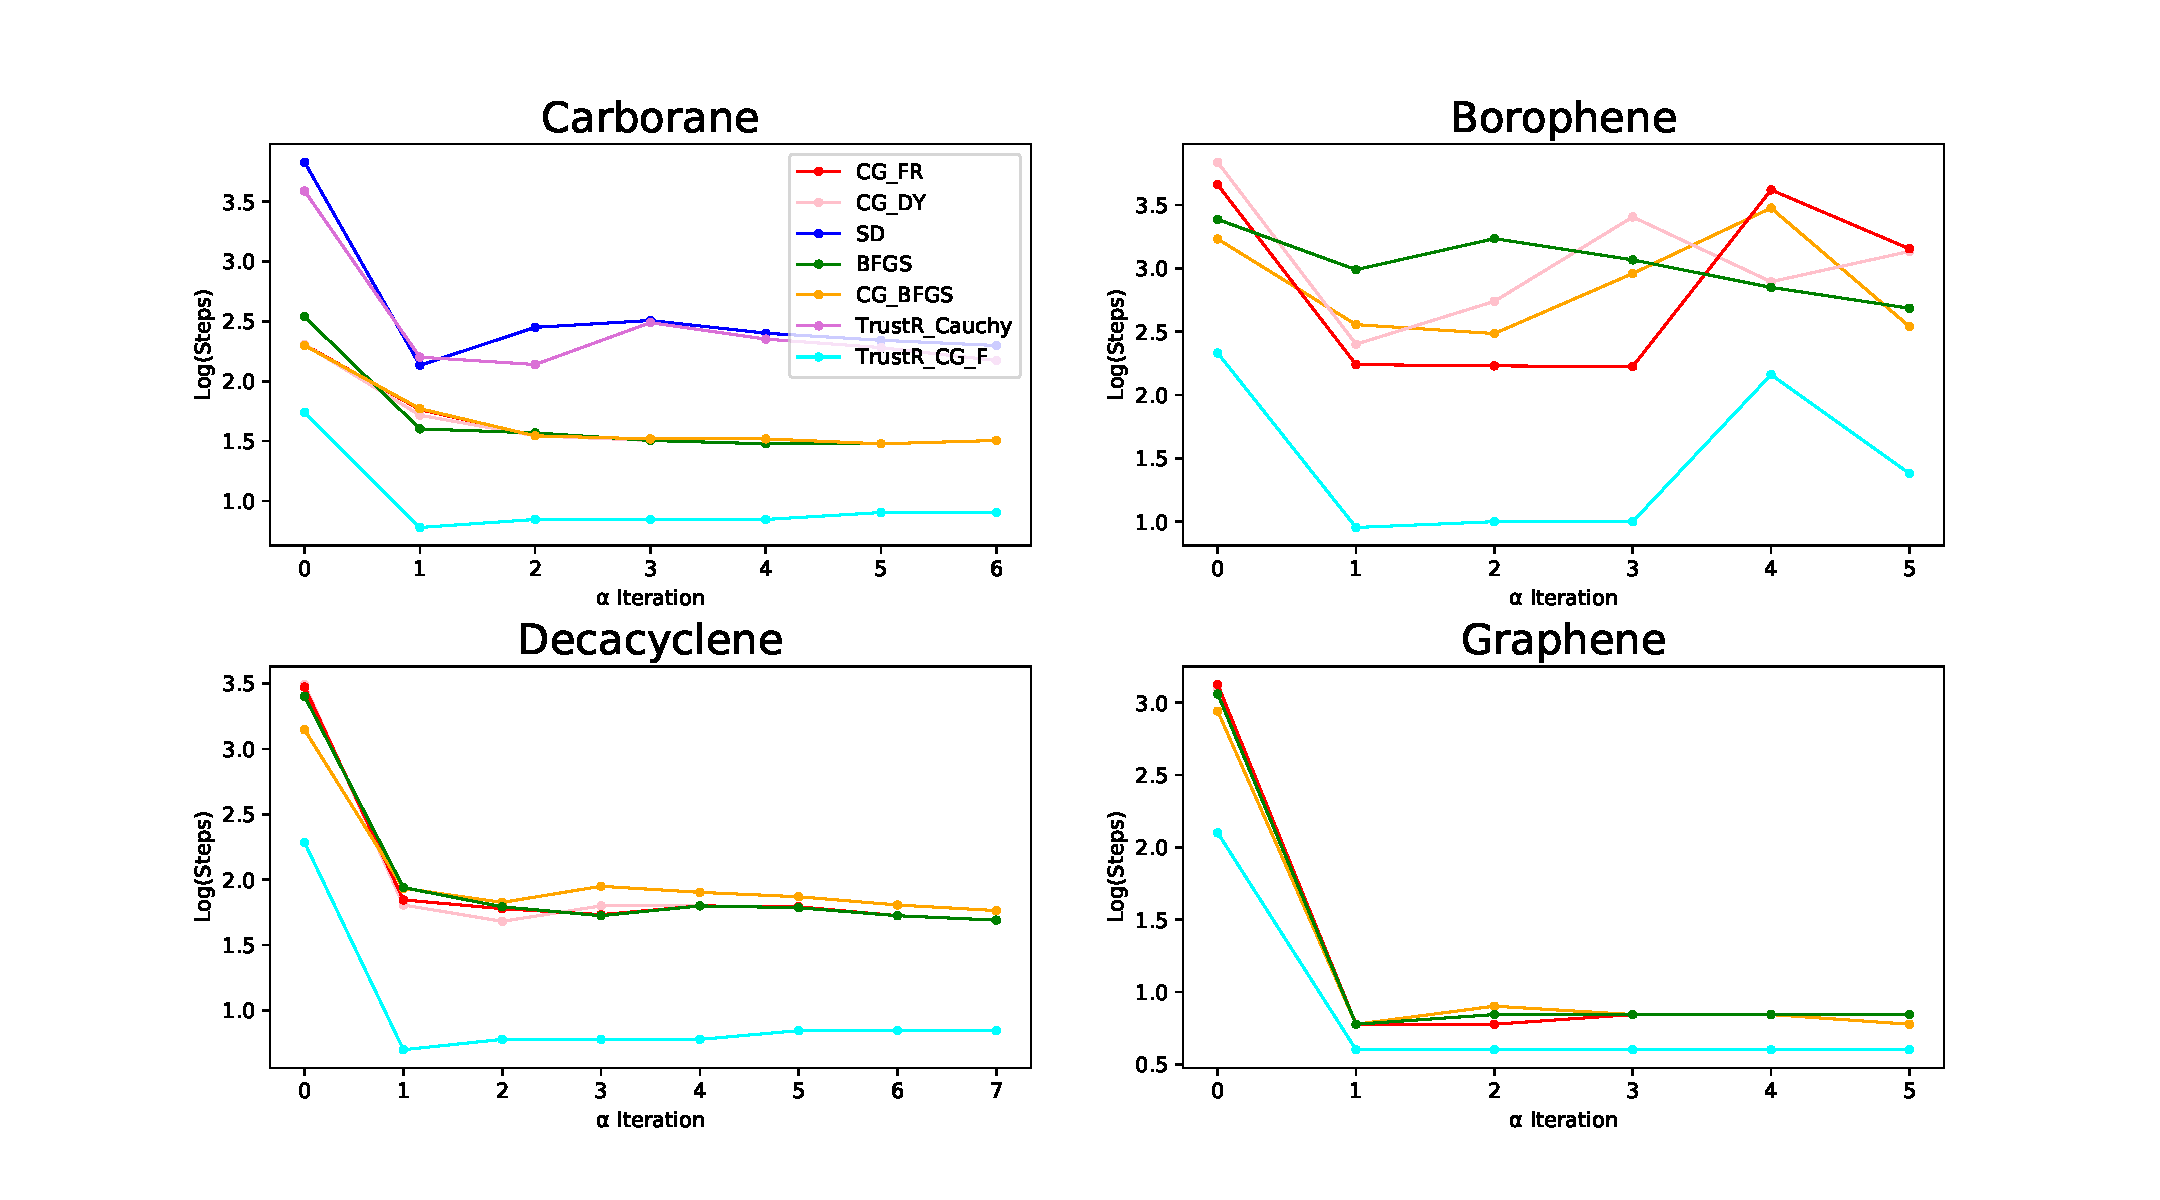
\includegraphics[width=\textwidth]{occupied_iter.pdf}
\caption{Total steps of each $\alpha$ iteration for occupied carborane, borophene, decacyclene and graphene systems}
\label{fig:occ_iter}
\end{figure*}


\begin{figure*}[htb]
\centering
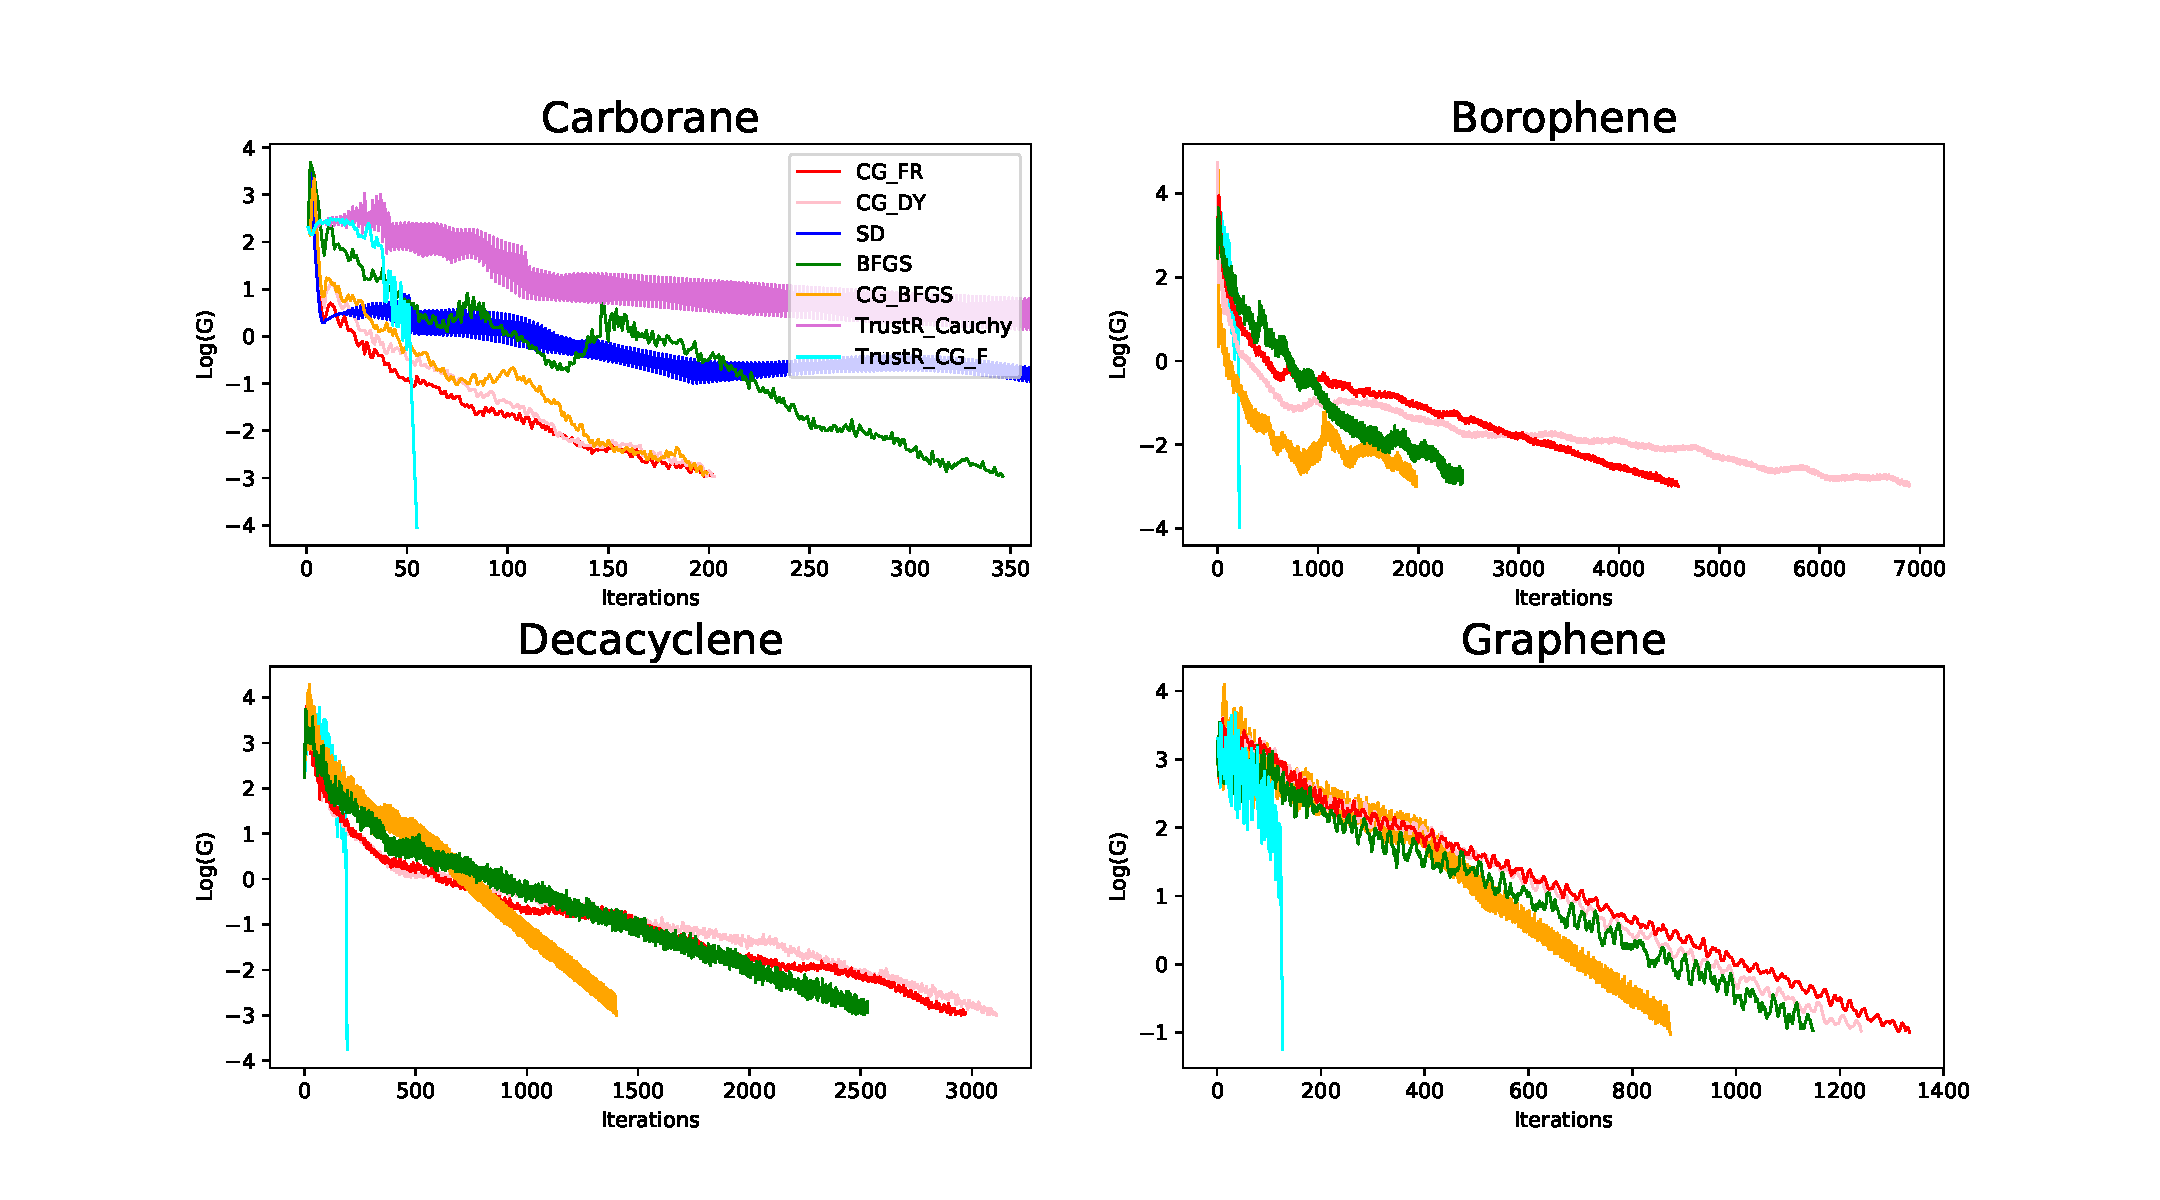
\includegraphics[width=\textwidth]{occupied_grad.pdf}
\caption{Performance of search direction schemes in the occupied Berghold localization of the MOs}
\label{fig:occ_grad}
\end{figure*}


\begin{figure*}[htb]
\centering
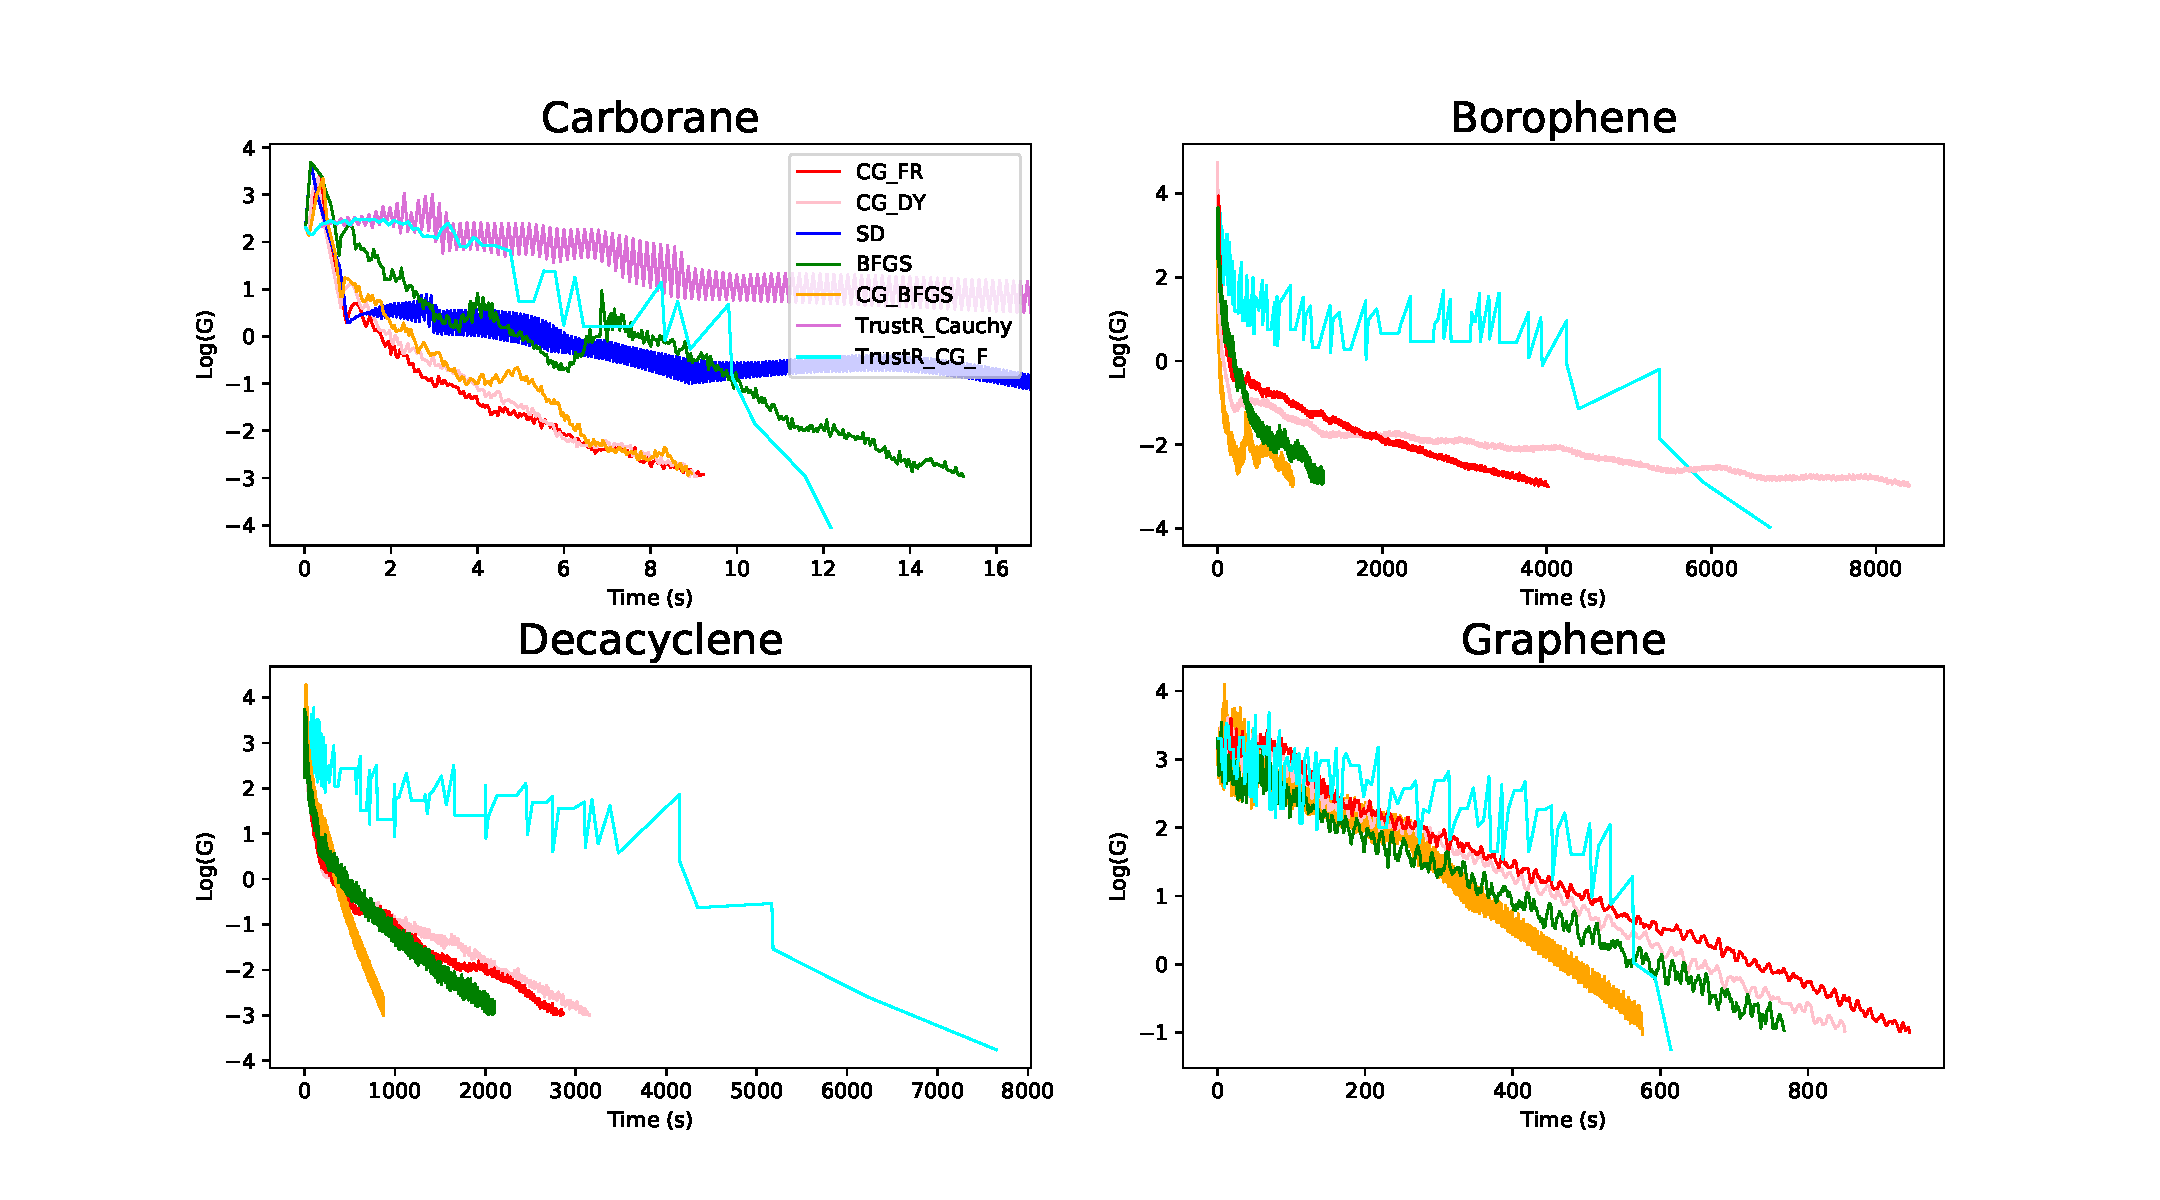
\includegraphics[width=\textwidth]{occupied_walltime.pdf}
\caption{Walltime comparison of the most time consuming $\alpha$ iteration in the occupied Berghold localization}
\label{fig:occ_walltime}
\end{figure*}


\begin{figure*}[htb]
\centering
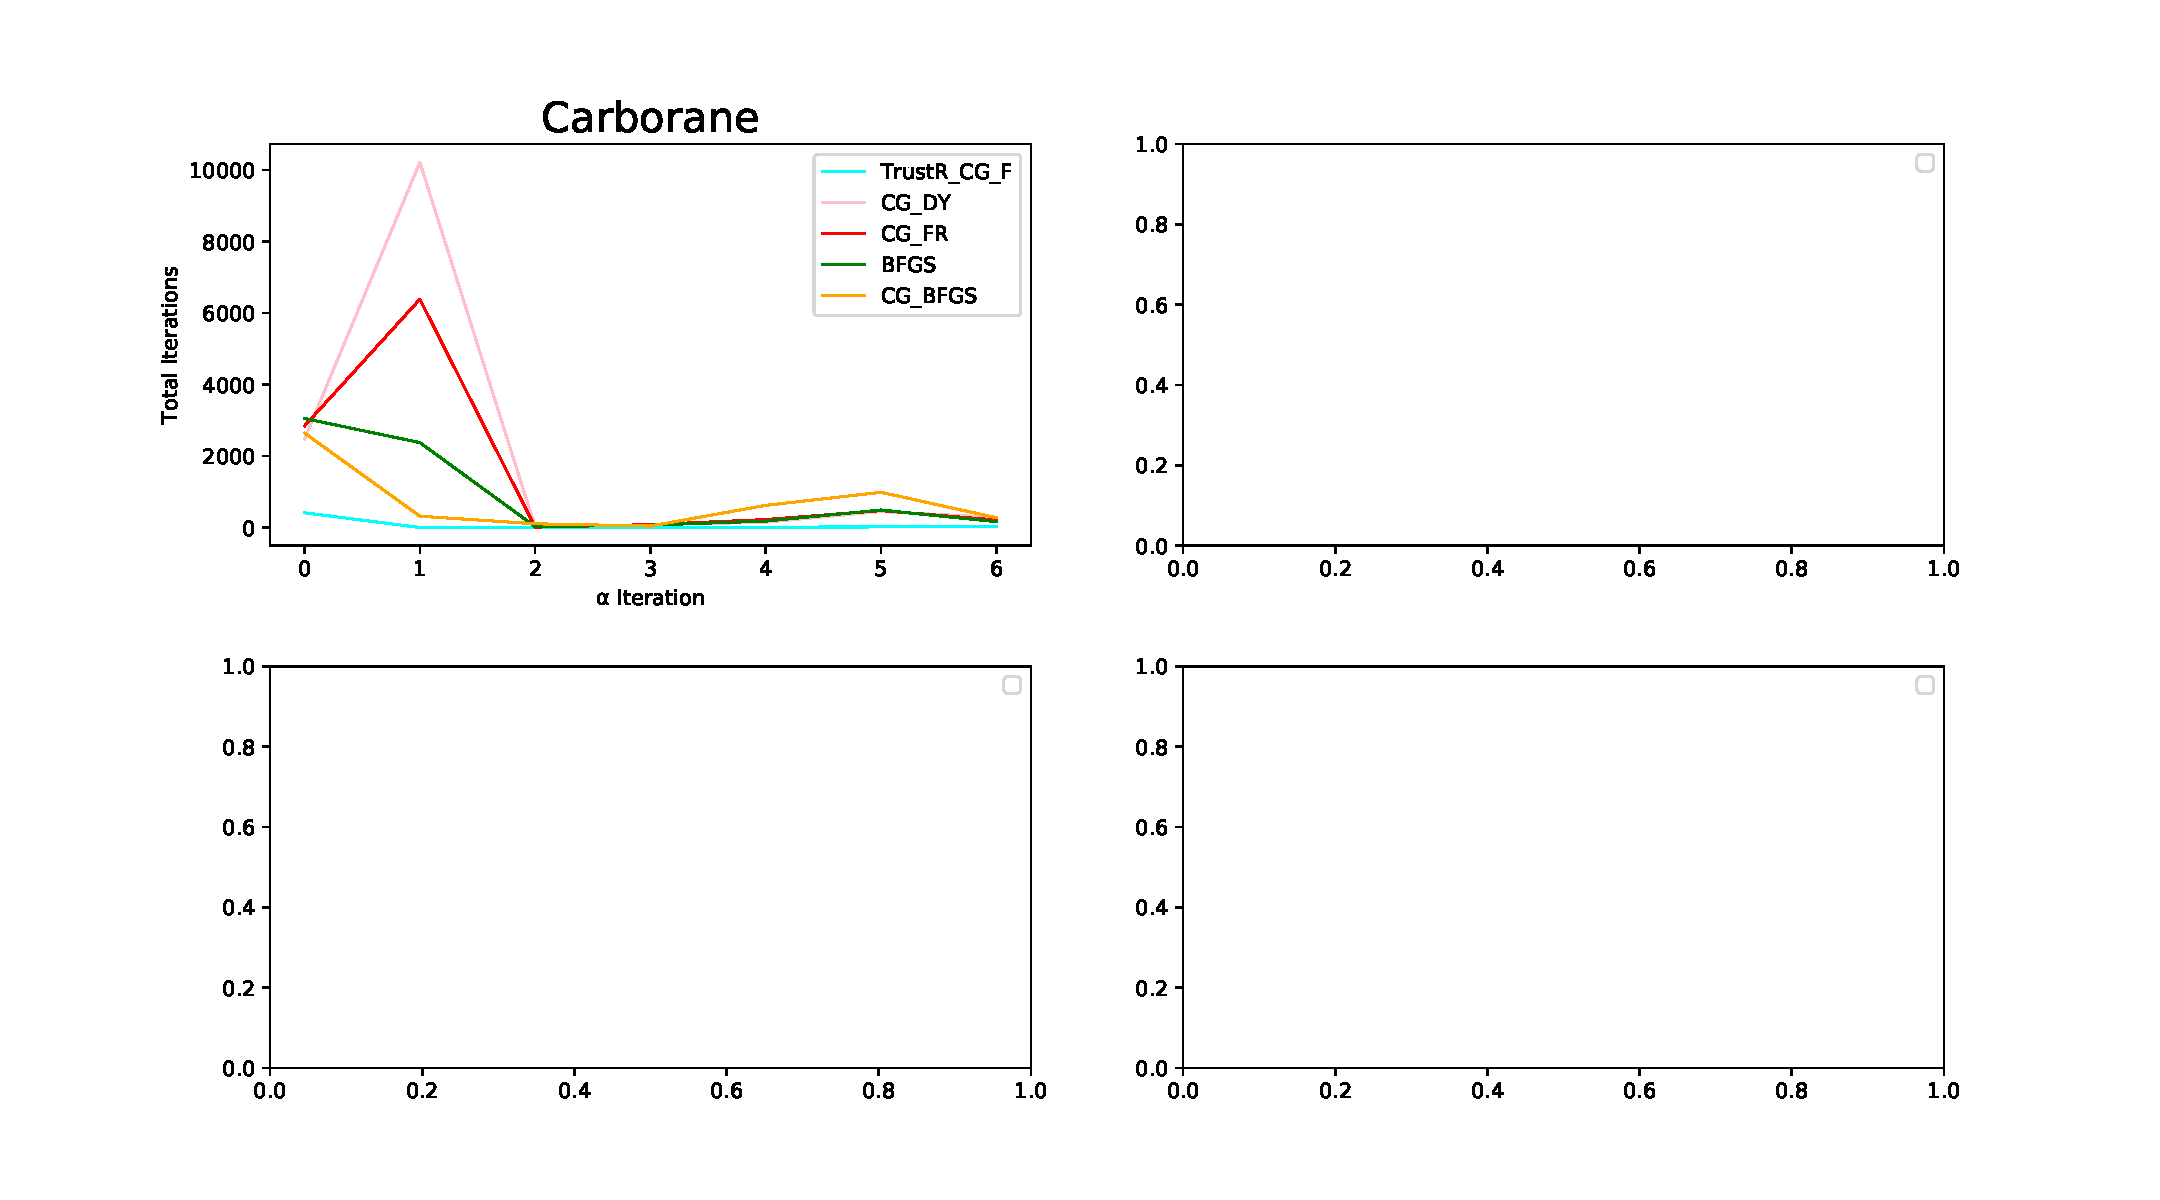
\includegraphics[width=\textwidth]{virtual_iter.pdf}
\caption{Total steps of each $\alpha$ iteration for virtual carborane, borophene, decacyclene and graphene systems}
\label{fig:vir_iter}
\end{figure*}

\begin{figure*}[htb]
\centering
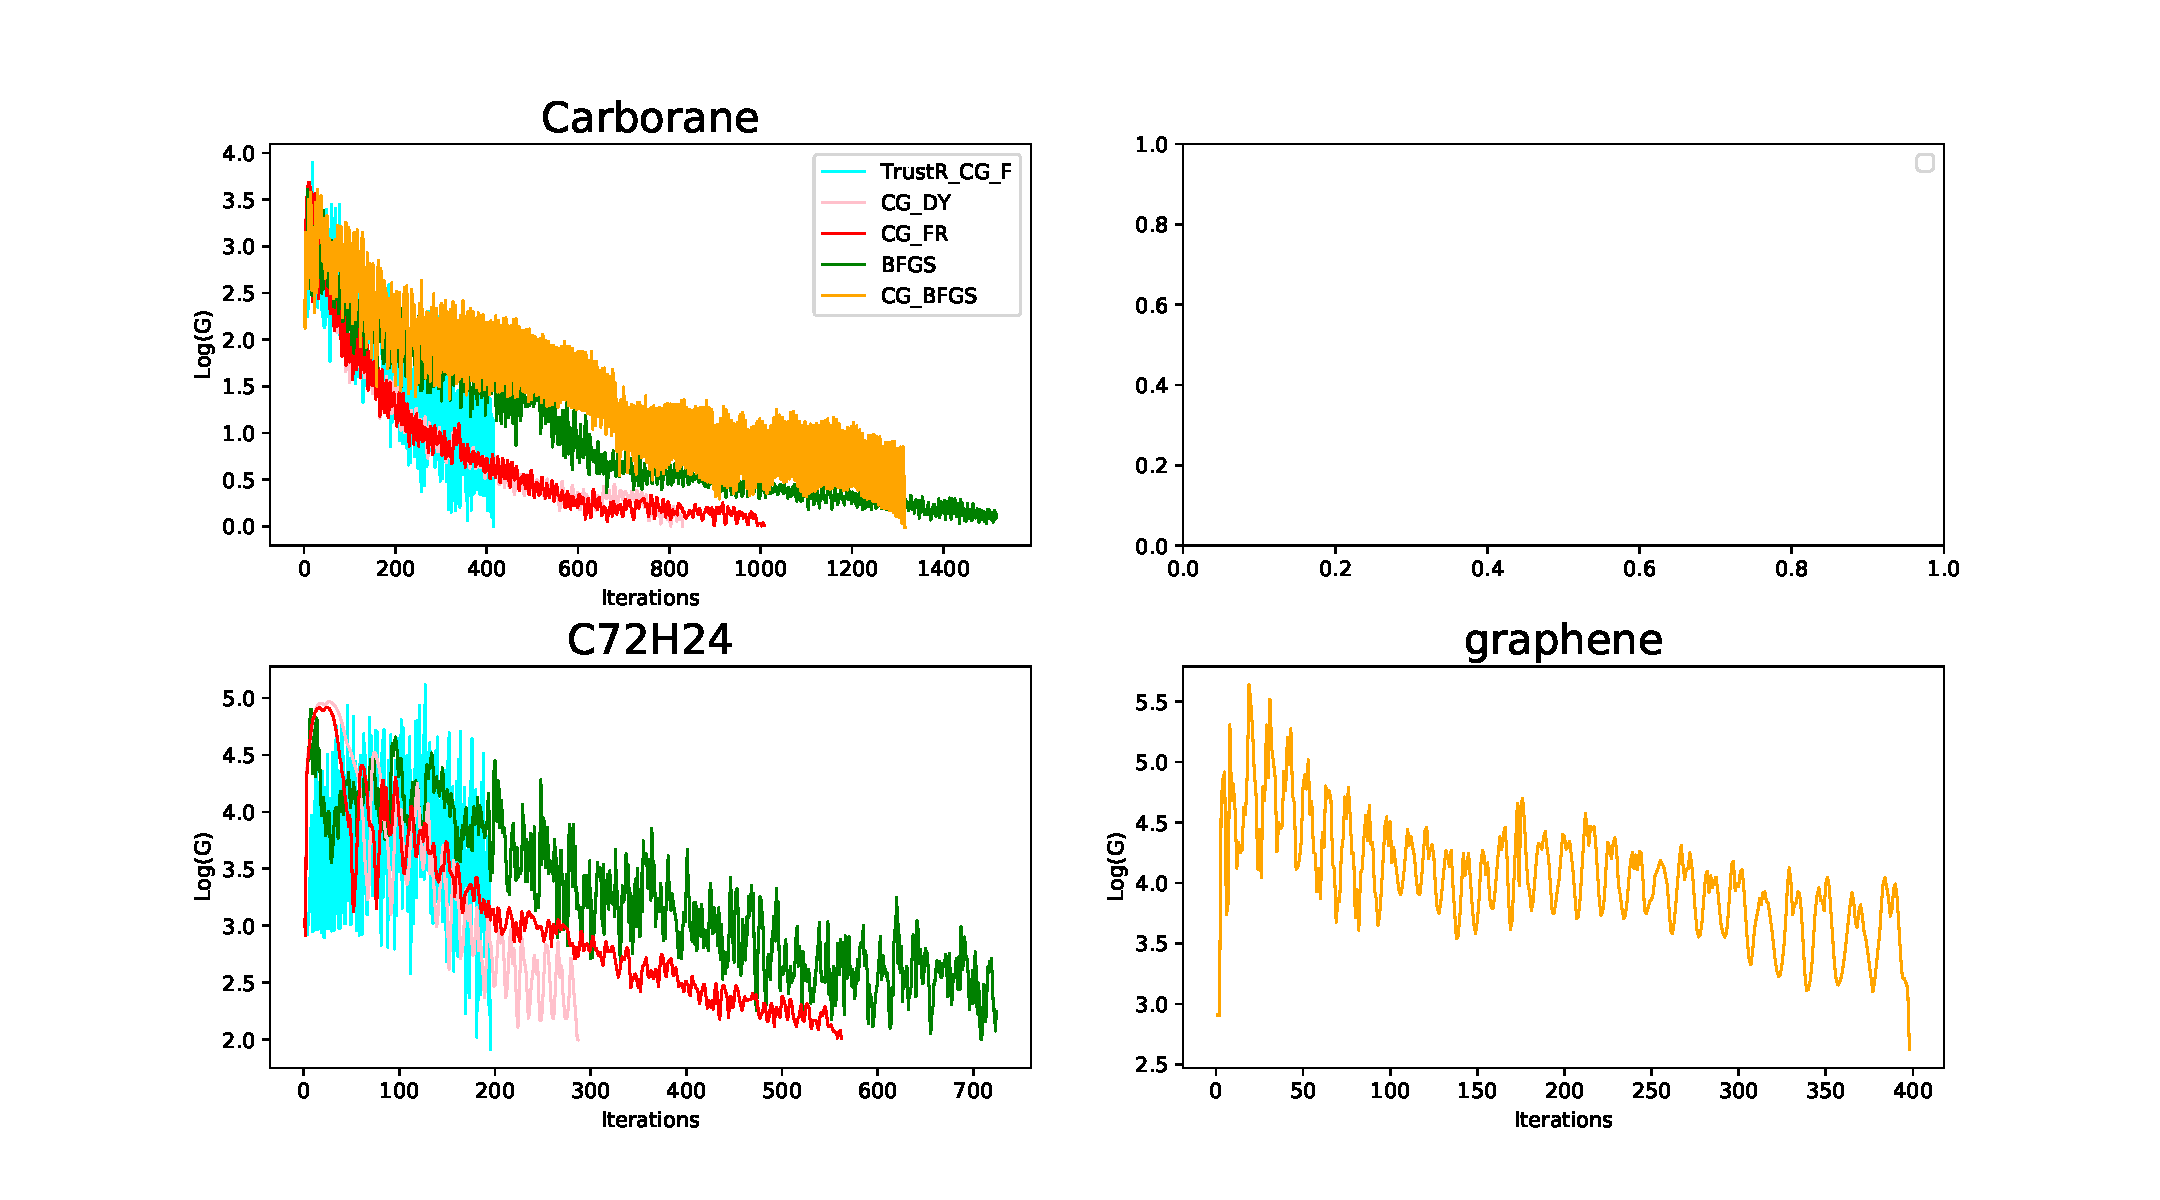
\includegraphics[width=\textwidth]{virtual_grad.pdf}
\caption{Performance of search direction schemes in the virtual Berghold localization of the MOs}
\label{fig:vir_grad}
\end{figure*}


\begin{figure*}[htb]
\centering
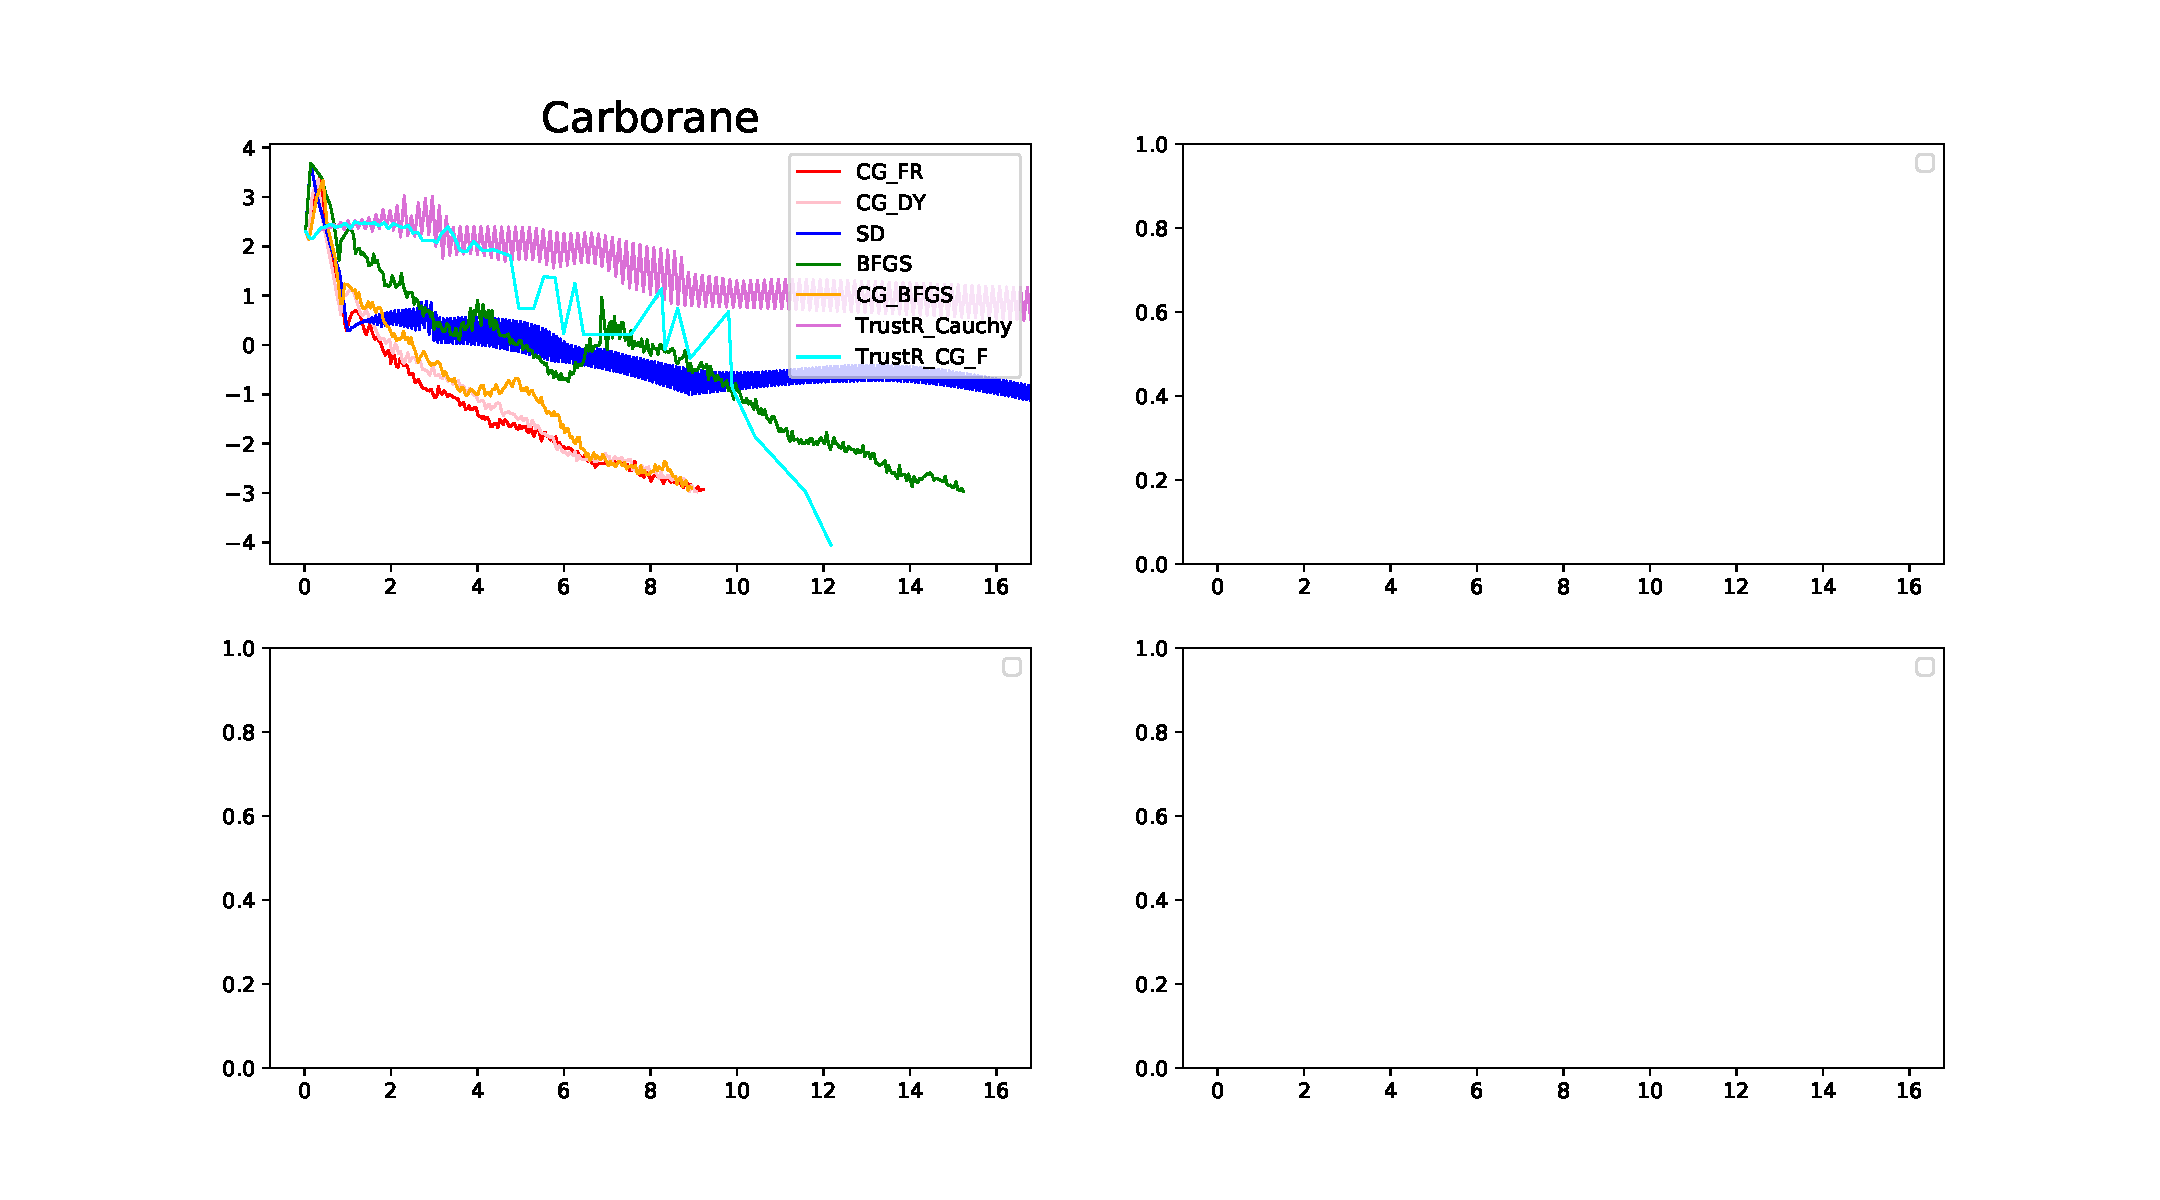
\includegraphics[width=\textwidth]{virtual_walltime.pdf}
\caption{Walltime comparison of the most time consuming $\alpha$ iteration in the virtual Berghold localization}
\label{fig:vir_walltime}
\end{figure*}


\section{Conclusions}

Questions:
1. Should we include newton method and Trust-region Dogleg?
2. Print out virtual orbitals
3. intel compiler and gfortran compiler, gfortran seems to work more efficient than intel in molecular systems?


\section{Acknowledgments} 


%\bibliographystyle{abbrv}
\bibliography{Virtuals,Virtuals-ctrl}

\end{document}

